\section{Results}\label{sec:results}

In order to evaluate the precision navigation system developed in this thesis, a number of different experiments, both on HARLIE and in simulation, were conducted. There were three major sets of experiments conducted: repeatability tests of the entire precision navigation system, tests to evaluate the acceptable initial conditions for phase space steering and tests to validate the splicing method used.

\subsection{Path Following Precision}\label{subsec:path_following_precision}

\begin{figure}
\centering
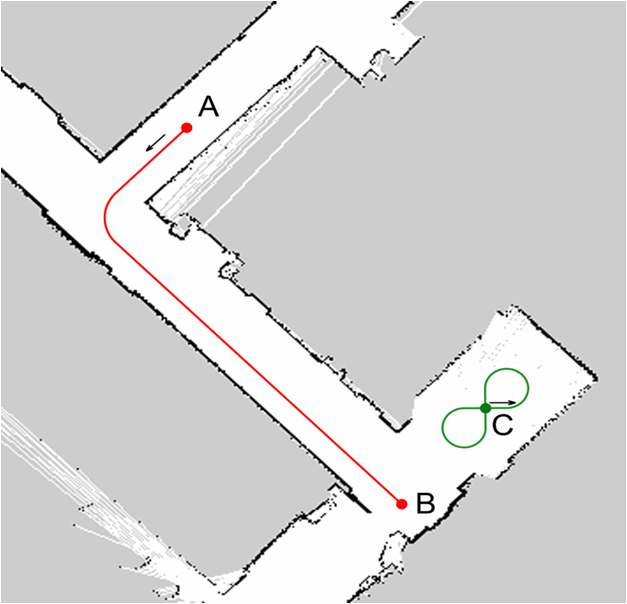
\includegraphics[width=0.75\textwidth]{images/path_following_paths}
\caption{Paths for Navigation Precision Tests \label{fig:path_following_paths}}
\end{figure}

The first set of tests run to evaluate the performance of the precision navigation system described in this thesis were designed to measure the actual precision with which it executed a path. To do this, two distinct sample paths were created on the second floor of the Case Western Reserve University Glennan building; these paths are shown overlaid to scale on the \emph{a priori} map in \autoref{fig:path_following_paths}. The first path, called the ``L'' path, is in red, which proceeds down a hallway from point A to point B. The second path, called the ``figure-8'' path, is in green. In the figure-8, the robot starts at point C facing in the direction indicated by the arrow and then proceeds around each arc before stopping again at point C. Throughout this section, a “run” on the L path refers to one complete trip starting at point A and ending at point B. For the figure-8 path, a “run” is defined as starting at point C, going through both the top and bottom loops and stopping again at point C. For the precision navigation system, both of these paths were described geometrically as a sequence of arcs and line segments.

To generate the path following performance measurements, five independent runs of the experiment were gathered while logging the pose of the robot with respect to the fixed origin of the \emph{a priori} map as estimated by the localization subsystem described in \autoref{sec:localization}. After all five runs were completed, the logged data was post-processed to compute lateral offsets relative to the desired path at each of the logged poses. The root-mean-square (RMS) of those lateral offsets was calculated for each individual run. This RMS value was averaged over all five runs of a given experiment and the standard deviation of those RMS values was calculated to generate a measure of repeatability.

\begin{figure}
\centering
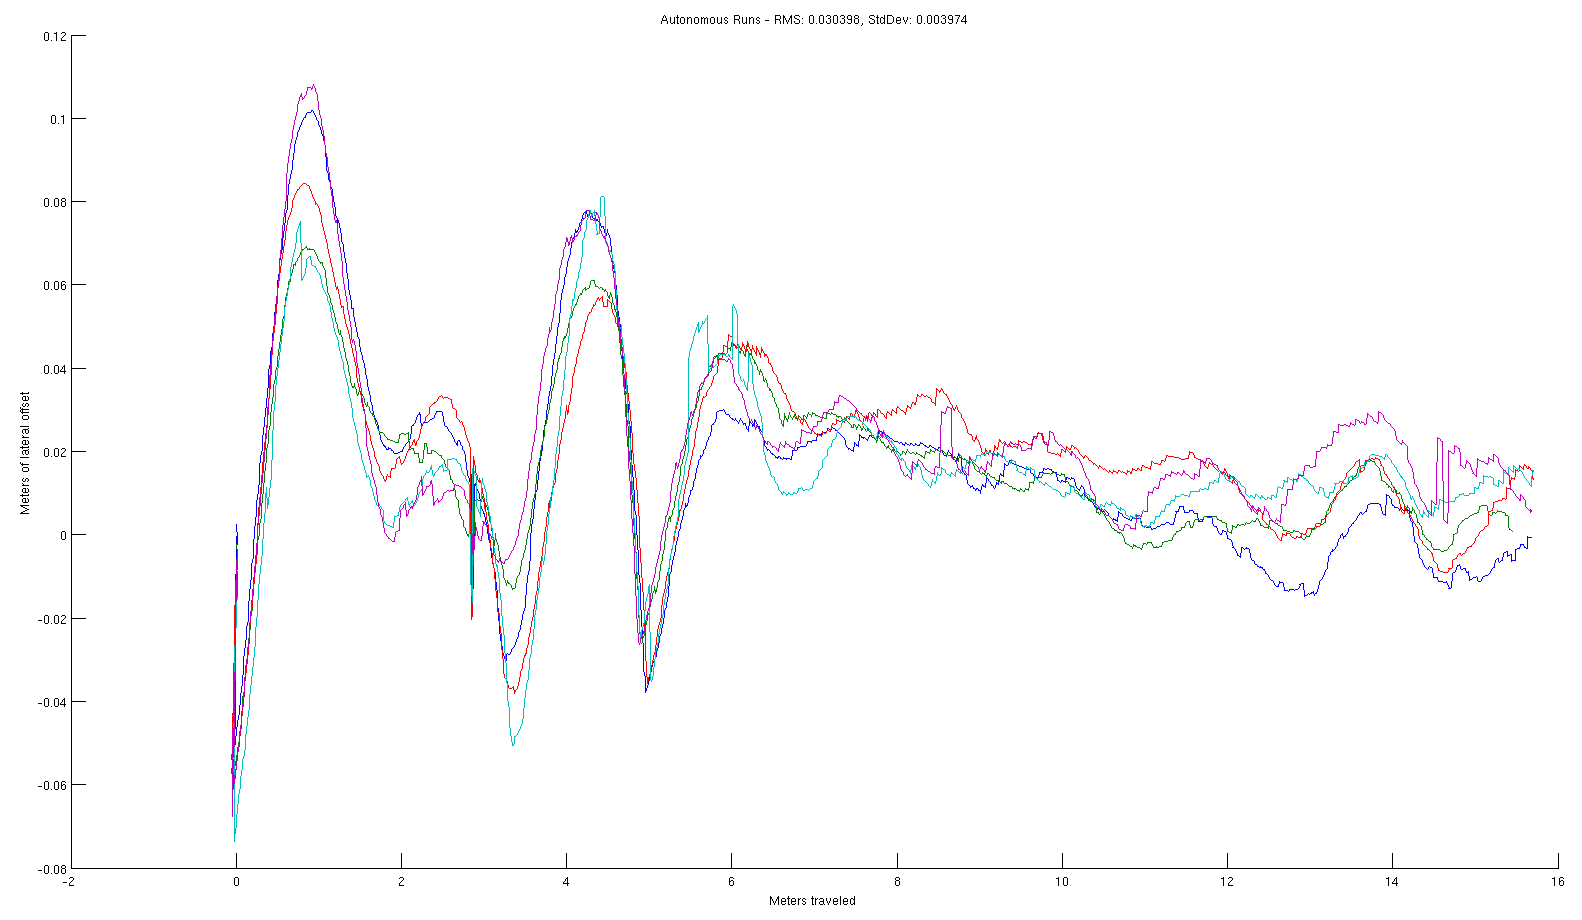
\includegraphics[width=0.95\textwidth]{images/l_path_autonomous_error}
\caption{Precision Navigation Error on the L Path \label{fig:l_path_autonomous_error}}{The X-axis is meters traveled and the Y-axis is meters of lateral offset}
\end{figure}

Performance was measured in terms of RMS lateral offsets from the defined path. \autoref{fig:l_path_autonomous_error} shows the performance of autonomous runs of the precision navigation system on the L path. As can be seen, the path following errors were small and highly repeatable. Lateral errors were just over three centimeters RMS, and this result was repeatable with a standard deviation of less than four millimeters.

\begin{figure}
\centering
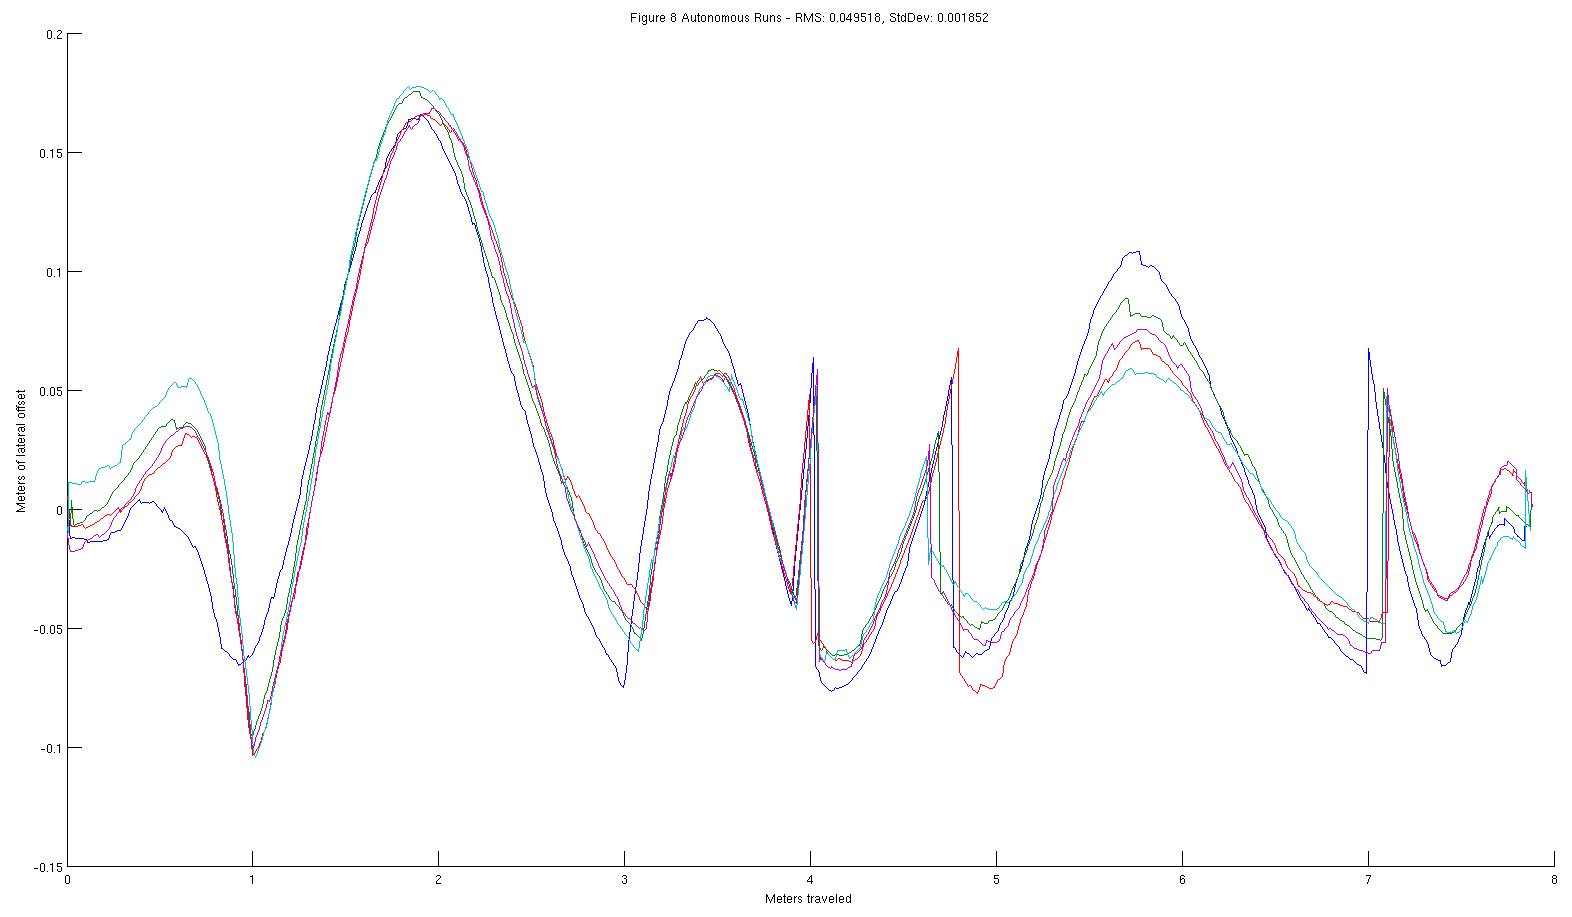
\includegraphics[width=0.95\textwidth]{images/fig_8_autonomous_error}
\caption{Precision Navigation Error on the Figure 8 Path \label{fig:fig_8_autonomous_error}}{The X-axis is meters traveled and the Y-axis is meters of lateral offset}
\end{figure}

The figure-8 test path had relatively tight turn radii (2ft), making it a more challenging path. Again, performance was measured in terms of RMS lateral offsets from the defined path. \autoref{fig:fig_8_autonomous_error} shows the performance of autonomous runs of the precision navigation system on the figure-8 path. As can be seen, the path following errors were small and highly repeatable. Lateral errors were less than five centimeters RMS, and this result was repeatable with a standard deviation of less than two centimeters.

The results for both of these tests show that the precision navigation described in this thesis is sufficiently precise for the use cases previously described, such as navigating a robotic wheelchair through an ADA-compliant doorway that would have under seven centimeters of clearance on either side of the robot. The majority of the lateral offset error shown in \autoref{fig:l_path_autonomous_error} and \autoref{fig:fig_8_autonomous_error} occurs at changes in the path curvatures. For example, in the L path error graph, the large variations in lateral offset at approximately one and four meters of distance traveled coincide with entering and leaving the arc between hallways. After leaving the arc (after approximately six meters traveled), the lateral offset error becomes much less variable as the robot reaches the long, straight section of the L path.

\subsection{Phase Space Steering Initial Condition Tests}\label{subsec:phase_space_steering_skills}

\subsection{Splicing Tests}\label{subsec:splicing_tests}

\begin{comment}

* Navigation on hallway and figure 8
* Joystick control results on same for comparison

* Skills
	* Door Skill
	* Tangent Skill

* Splicing

\end{comment}